\section{Sistema de adquisición}
\label{sec:diseno}

La aplicación del método exige convertir el movimiento vertical del terreno en una señal eléctrica sin perder la relación temporal entre posiciones. Esa tarea comienza en el receptor disponible y continúa en una cadena de acondicionamiento, conversión y almacenamiento. El sistema separa el nodo GEO, conectado al geófono, el nodo HAMMER, conectado al martillo instrumentado, y un maestro que coordina la sesión. Cada nodo conserva localmente la captura y sus parámetros; la comunicación transporta órdenes y resultados, pero no forma parte del lazo temporal de muestreo.

\begin{figure*}[!tb]
\centering
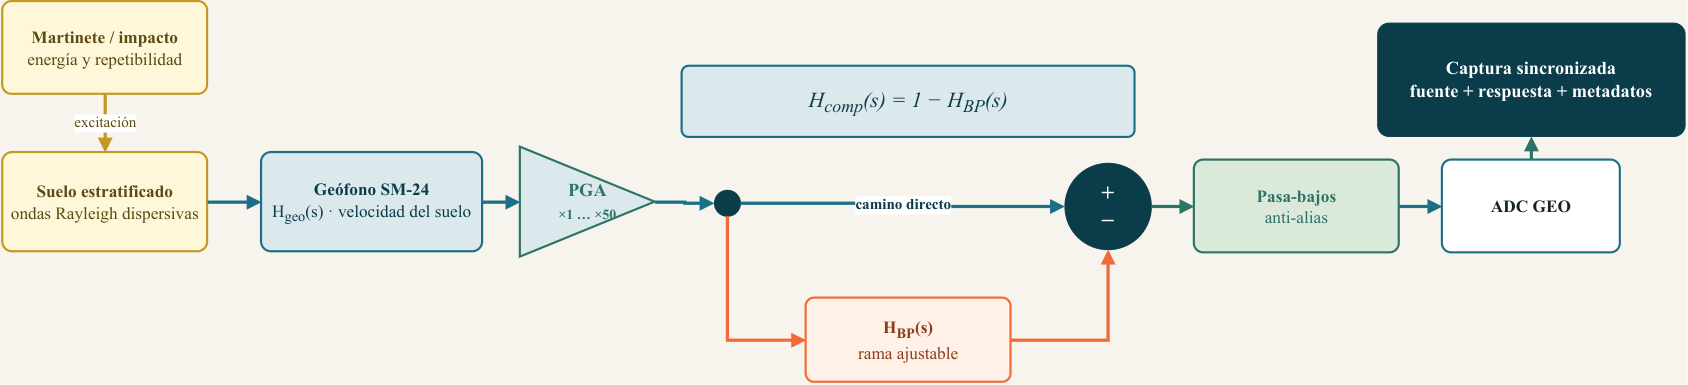
\includegraphics[width=0.94\textwidth,keepaspectratio]{d_cadena_fuente_geofono.png}
\caption{Cadena funcional de medida: el impacto excita el terreno, el geófono transforma el movimiento vertical y la electrónica acondiciona, digitaliza y conserva la traza.}
\label{fig:cadena-medida}
\end{figure*}

\subsection{Requerimientos derivados de la medida}

\textbf{Banda y fase.} Las longitudes de onda mayores corresponden a frecuencias menores; por ello la banda baja condiciona el alcance. La cadena debe evitar introducir variaciones de fase no conocidas dentro de la banda analizada y debe registrar a una frecuencia suficiente para impedir aliasing temporal.

\textbf{Margen dinámico.} La señal cercana a la fuente puede coexistir con respuestas atenuadas en posiciones lejanas. Se requiere ganancia programable por captura, protección frente a saturación y resolución suficiente para conservar las trazas débiles.

\textbf{Referencia temporal y geometría.} Cada muestra debe quedar referida al golpe y cada archivo debe conservar posición, ganancia, frecuencia de muestreo y versión del hardware. En una operación futura con varios nodos también deberá verificarse el error relativo de sus bases de tiempo.

\textbf{Operación de campo.} El instrumento debe trabajar sin infraestructura externa, almacenar una copia local y permitir revisar inmediatamente si el golpe y la respuesta fueron captados antes de abandonar la posición. Estos requerimientos traducen al instrumento las condiciones de adquisición y control de calidad recomendadas para ensayos de ondas superficiales \citep{Foti2018}.

\subsection{Geófono utilizado}
\label{sec:geofono}

El receptor disponible es un geófono vertical pasivo SM-24, de frecuencia natural nominal \SI{10}{Hz}, sensibilidad \SI{28.8}{V.s/m} y amortiguamiento dependiente de la carga \citep{SM24}. No fue elegido porque represente el transductor ideal, sino porque se encontraba disponible y permitía construir el primer canal sin adquirir un sensor de banda ancha. Esta restricción material define el problema electrónico: por debajo de su resonancia, la tensión entregada disminuye rápidamente respecto del movimiento del terreno, justamente en la región asociada con longitudes de onda mayores.

Geófonos de menor frecuencia natural o sismómetros de banda ancha reducirían esa dificultad, pero cada posición simultánea exigiría un transductor adicional. Como referencia de orden, los precios públicos consultados sitúan el SM-24 alrededor de 70 USD y un geófono vertical de 4,5 Hz entre 92 y 154 USD por elemento, antes de incorporar el resto del canal \citep{SparkFunSM24,RTClark45}. El proyecto ensaya otra vía: caracterizar el SM-24 disponible y extender de manera controlada su banda útil mediante acondicionamiento.

\begin{figure*}[!tb]
\centering
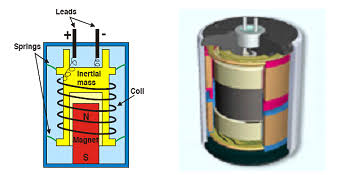
\includegraphics[width=0.40\textwidth]{f_geofono_interior.png}\hfill
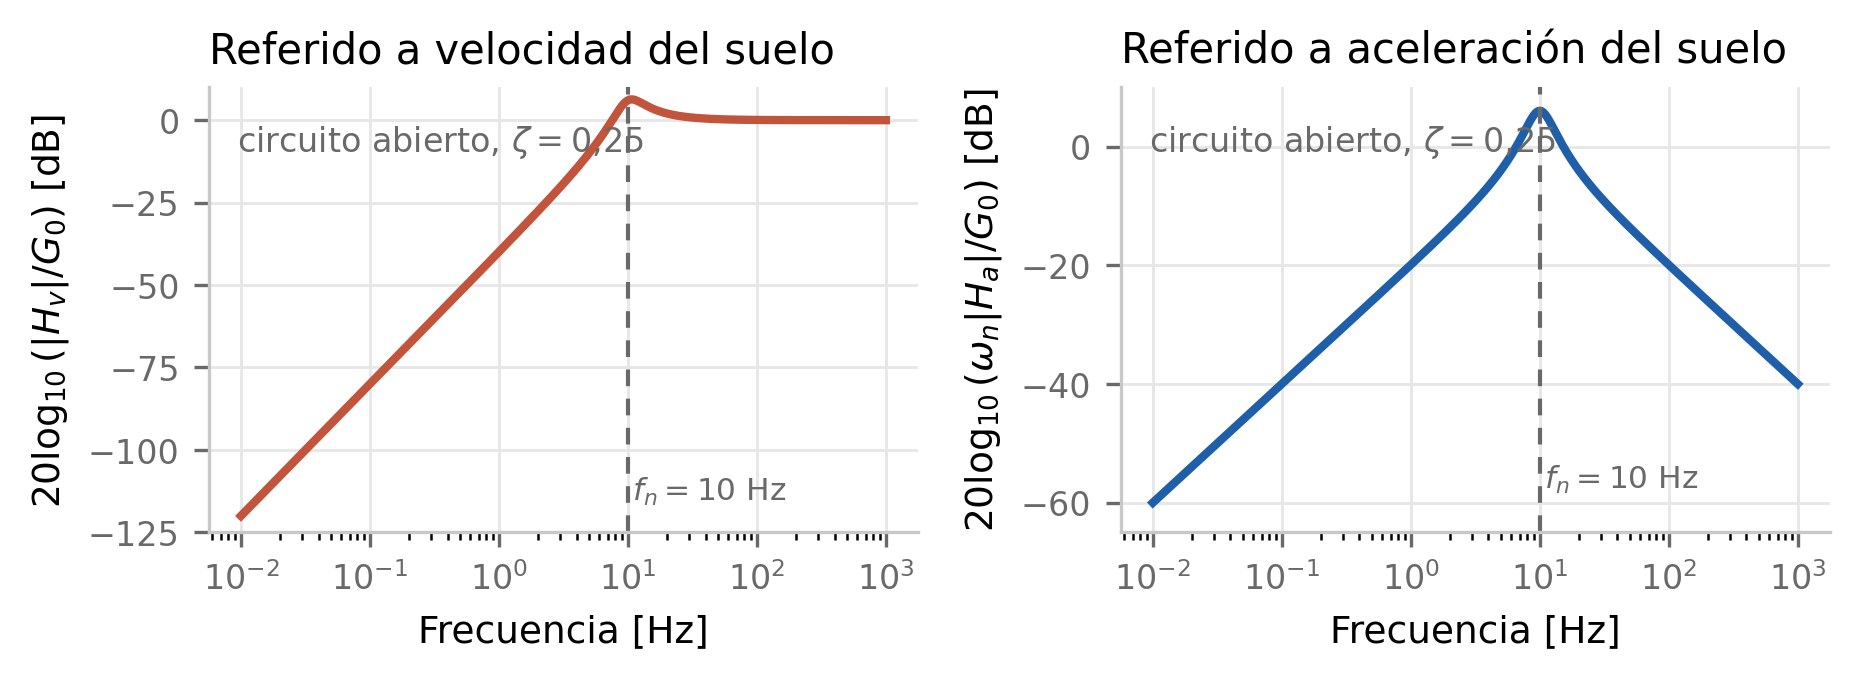
\includegraphics[width=0.54\textwidth]{respuesta_sm24_modelo.png}
\caption{Izquierda: principio del geófono de bobina móvil. Derecha: respuesta nominal del SM-24 referida a velocidad y aceleración del terreno. Fuentes: ilustración del principio reproducida de \citet{Breslin2020} y modelo elaborado a partir de \citet{SM24}.}
\label{fig:geofono-respuesta}
\end{figure*}

Si $x_g$ es el desplazamiento del chasis solidario al suelo y $u=x_m-x_g$ el desplazamiento relativo de la masa, el equilibrio mecánico es
\begin{equation}
m\ddot u+c\dot u+ku=-m\ddot x_g.
\label{eq:geofono-mecanico}
\end{equation}
donde $m$ es la masa móvil, $c$ reúne el amortiguamiento mecánico y eléctrico, y $k$ representa la rigidez de la suspensión. Con $\omega_n=\sqrt{k/m}$ y $\zeta=c/(2m\omega_n)$, y considerando que la tensión inducida es proporcional a $\dot u$, la respuesta respecto de la velocidad del terreno adopta la forma de un sistema de segundo orden pasa-altos. Lejos por encima de $\omega_n$ la salida es aproximadamente proporcional a velocidad; por debajo, la atenuación crece. La electrónica no crea energía ausente en la excitación, pero puede evitar que la respuesta del sensor y el acondicionamiento agraven innecesariamente esa pérdida.

Si $G_0$ es la sensibilidad electromecánica, la salida es $V_o=G_0\dot u$. Con condiciones iniciales nulas, la respuesta referida a la aceleración del terreno $A_g(s)$ queda
\begin{equation}
H_a(s)=\frac{V_o(s)}{A_g(s)}=
-G_0\frac{s}{s^2+2\zeta_0\omega_n s+\omega_n^2}.
\label{eq:geofono-aceleracion}
\end{equation}
Esta forma pasabanda es la base de la compensación. El amortiguamiento $\zeta_0$ incluye pérdidas mecánicas y eléctricas; por ello la impedancia de entrada del frente también carga la bobina y modifica la respuesta. La entrada se diseñó con impedancia alta y simétrica para no introducir una carga diferente entre unidades \citep{SM24,Ma2023}.

\subsection{Frente analógico}
\label{sec:afe}

El frente se implementó dentro de un PSoC y organiza cinco funciones: entrada diferencial, ganancia programable, rama pasabanda de compensación, suma con el camino directo y filtrado antialias. La entrada diferencial rechaza perturbaciones comunes en el cable del geófono. La etapa PGA adapta el nivel a la captura sin fijar una única ganancia para todas las distancias.

\begin{figure*}[!tb]
\centering
\includegraphics[width=\textwidth,keepaspectratio]{f_frente_analogico.png}
\caption{Frente analógico implementado: entrada diferencial, ganancia programable, rama pasabanda ajustable, sumador y filtro pasa-bajos anterior al ADC. Se reproduce el esquemático completo. Fuente: elaboración propia en PSoC Creator.}
\label{fig:frente-analogico}
\end{figure*}

\begin{table*}[!tb]
\centering
\footnotesize
\caption{Lectura funcional del esquemático completo de la figura~\ref{fig:frente-analogico}.}
\begin{tabularx}{0.96\textwidth}{@{}lYYY@{}}
\toprule
Etapa & Entrada y salida & Función & Parámetros esenciales \\
\midrule
Entrada y PGA & SM-24 diferencial $\rightarrow$ PGA & Rechazo de modo común y adaptación de nivel & Entrada simétrica; ganancia $\times1$ a $\times50$ \\
Pasabanda (BP) & Copia del PGA $\rightarrow$ rama BP & Generar la contribución correctora bajo resonancia & Centro próximo a \SI{10.2}{Hz}; potenciómetro digital \\
Sumador & Camino directo y BP $\rightarrow$ SUM & Combinar rutas y recuperar nivel & Aproximadamente $\times3.6$ en la rama compensada \\
Pasa-bajos (LP) & SUM $\rightarrow$ LP & Limitar contenido antes del muestreo & Topología MFB; ganancia aproximada $\times5$ \\
MUX y ADC & PGA, BP, SUM o LP $\rightarrow$ ADC & Observar etapas, calibrar y digitalizar & VDAC por etapa; ADC delta--sigma \\
\bottomrule
\end{tabularx}
\label{tab:lectura-afe}
\end{table*}

Una deconvolución exacta de la respuesta del geófono amplificaría junto con la señal el ruido de baja frecuencia. Por ello se adopta el principio de \citet{Ma2023}: conservar la frecuencia natural y aumentar el amortiguamiento efectivo para aplanar, en una banda limitada, la respuesta referida a aceleración por debajo de la resonancia. La implementación es analógica: una copia pasabanda de la salida se combina con el camino directo. El resultado queda atenuado y debe recuperarse mediante ganancia. Un potenciómetro digital ajusta la proporción de la rama pasabanda para compensar tolerancias y acercar la respuesta de distintos nodos sin suponer que sean idénticos.

El compensador ideal transforma el amortiguamiento nominal $\zeta_0$ en un valor mayor $\zeta_1$:
\begin{equation}
H_{\mathrm{comp}}(s)=
\frac{s^2+2\zeta_0\omega_n s+\omega_n^2}
{s^2+2\zeta_1\omega_n s+\omega_n^2}.
\label{eq:compensador}
\end{equation}
Al separar el término constante se obtiene una ruta directa menos una contribución pasabanda:
\begin{equation}
H_{\mathrm{comp}}(s)=1-
\frac{2(\zeta_1-\zeta_0)\omega_n s}
{s^2+2\zeta_1\omega_n s+\omega_n^2}.
\label{eq:compensador-separado}
\end{equation}
La arquitectura implementa físicamente esas dos rutas. Para el bajo factor de calidad requerido, la rama inversora emplea un par $RC$ en la entrada y otro en la realimentación. Sus quiebres ideales son
\begin{equation}
f_{\mathrm{low}}=\frac{1}{2\pi R_{\mathrm{in}}C_{\mathrm{in}}},
\qquad
f_{\mathrm{high}}=\frac{1}{2\pi R_{\mathrm f}C_{\mathrm f}}.
\label{eq:quiebres}
\end{equation}
Los valores se buscaron sobre componentes comerciales incorporando el modelo no ideal del amplificador. El potenciómetro se dejó como grado de libertad de calibración porque la cancelación depende de relaciones reales, no sólo de valores nominales.

Con los valores implementados se obtiene una frecuencia central próxima a \SI{10.2}{Hz} y un amortiguamiento efectivo de diseño $\zeta_1\simeq937$. La respuesta compensada queda fuertemente atenuada y esa pérdida debe recuperarse con ganancia. Para evitar concentrar el margen en un único bloque, se distribuyó entre entrada instrumental ($\times2$), PGA ($\times1$ a $\times50$), sumador ($\times3{,}6$ en la rama compensada) y pasa-bajos ($\times5$). El producto máximo es cercano a $\times1800$. Este reparto explica por qué los offsets y el ruido de cada etapa requieren atención específica.

La etapa final limita la banda antes del convertidor. Se utilizó una topología de realimentación múltiple: las etapas previas ya presentan baja impedancia de salida y no se necesita la alta impedancia de entrada característica de otras alternativas. La frecuencia de corte y la tasa de muestreo se seleccionan en conjunto; el filtro analógico reduce el contenido que podría plegarse y el procesamiento digital restringe después la banda usada por el análisis.

La ganancia no se fija globalmente para toda una campaña. El operador puede seleccionar una configuración por posición después de observar una captura de prueba. La regla es ocupar una fracción alta del rango sin recortar el primer arribo ni el impacto transmitido por acoplamientos eléctricos o mecánicos. El valor elegido se almacena como metadato; normalizar después las trazas no recuperaría una señal saturada ni corregiría un cambio de fase desconocido.

\subsection{Por qué la compensación exige calibrar la continua}
\label{sec:calibracion}

La ganancia necesaria para recuperar la rama compensada también amplifica los errores de continua. Los amplificadores operacionales integrados en el PSoC 5LP no son dispositivos de deriva nula: presentan tensión de offset y variación con temperatura, y cada etapa suma su contribución a la siguiente \citep{InfineonPSoC,InfineonAN68403}. Sin corrección, una salida puede acercarse a un riel aun con el geófono en reposo y consumir el margen que debía reservarse para la señal. La compensación de baja frecuencia conduce así, de manera directa, a un segundo requisito: calibrar la continua antes de cada adquisición relevante.

El propio PSoC aporta los recursos para cerrar esa calibración. Un multiplexor lleva al ADC las salidas de PGA, pasabanda, sumador y pasa-bajos; los convertidores digital--analógico VDAC ajustan las referencias de cada etapa y el procesador coordina la secuencia \citep{InfineonPSoC,InfineonAN68403}. Durante la calibración se reutiliza el filtro digital programable como estimador de continua FIR de 128 coeficientes, máximo disponible en el bloque implementado. Para la etapa $i$ se calcula
\begin{equation}
\bar y_i[n]=\frac{1}{128}\sum_{r=0}^{127}y_i[n-r],
\qquad e_i[n]=r_i-\bar y_i[n],
\label{eq:estimador-dc}
\end{equation}
y el código del VDAC se corrige mediante una acción proporcional--integral discreta,
\begin{equation}
d_i[n+1]=d_i[n]+K_{P,i}\bigl(e_i[n]-e_i[n-1]\bigr)+K_{I,i}e_i[n].
\label{eq:pi-calibracion}
\end{equation}
Con el geófono en reposo se recorre cada etapa, se ajusta su referencia y sólo después se habilita la siguiente. La calibración se ejecuta antes de cada campaña. Durante la adquisición los controladores quedan desactivados y los códigos permanecen constantes, evitando que un lazo lento modifique la señal medida.

Fuera de una banda muerta, el controlador actualiza el código; dentro de ella se exige permanencia durante un número mínimo de muestras. La saturación suspende la integración en la dirección que empeoraría el error. Este tratamiento evita oscilaciones alrededor de la referencia y limita el tiempo de búsqueda.

El orden PGA, pasabanda, sumador y pasa-bajos es obligatorio porque corregir una etapa cambia el nivel de continua que reciben las siguientes. Entre etapas se reinicia el FIR y se espera su asentamiento. Al finalizar se prueba un código vecino y se conserva sólo si reduce el residuo. Los valores válidos se guardan por configuración de ganancia en EEPROM junto con versión, máscara de validez y CRC. Una corrida fallida no reemplaza una calibración anterior válida.

\begin{figure*}[!tb]
\centering
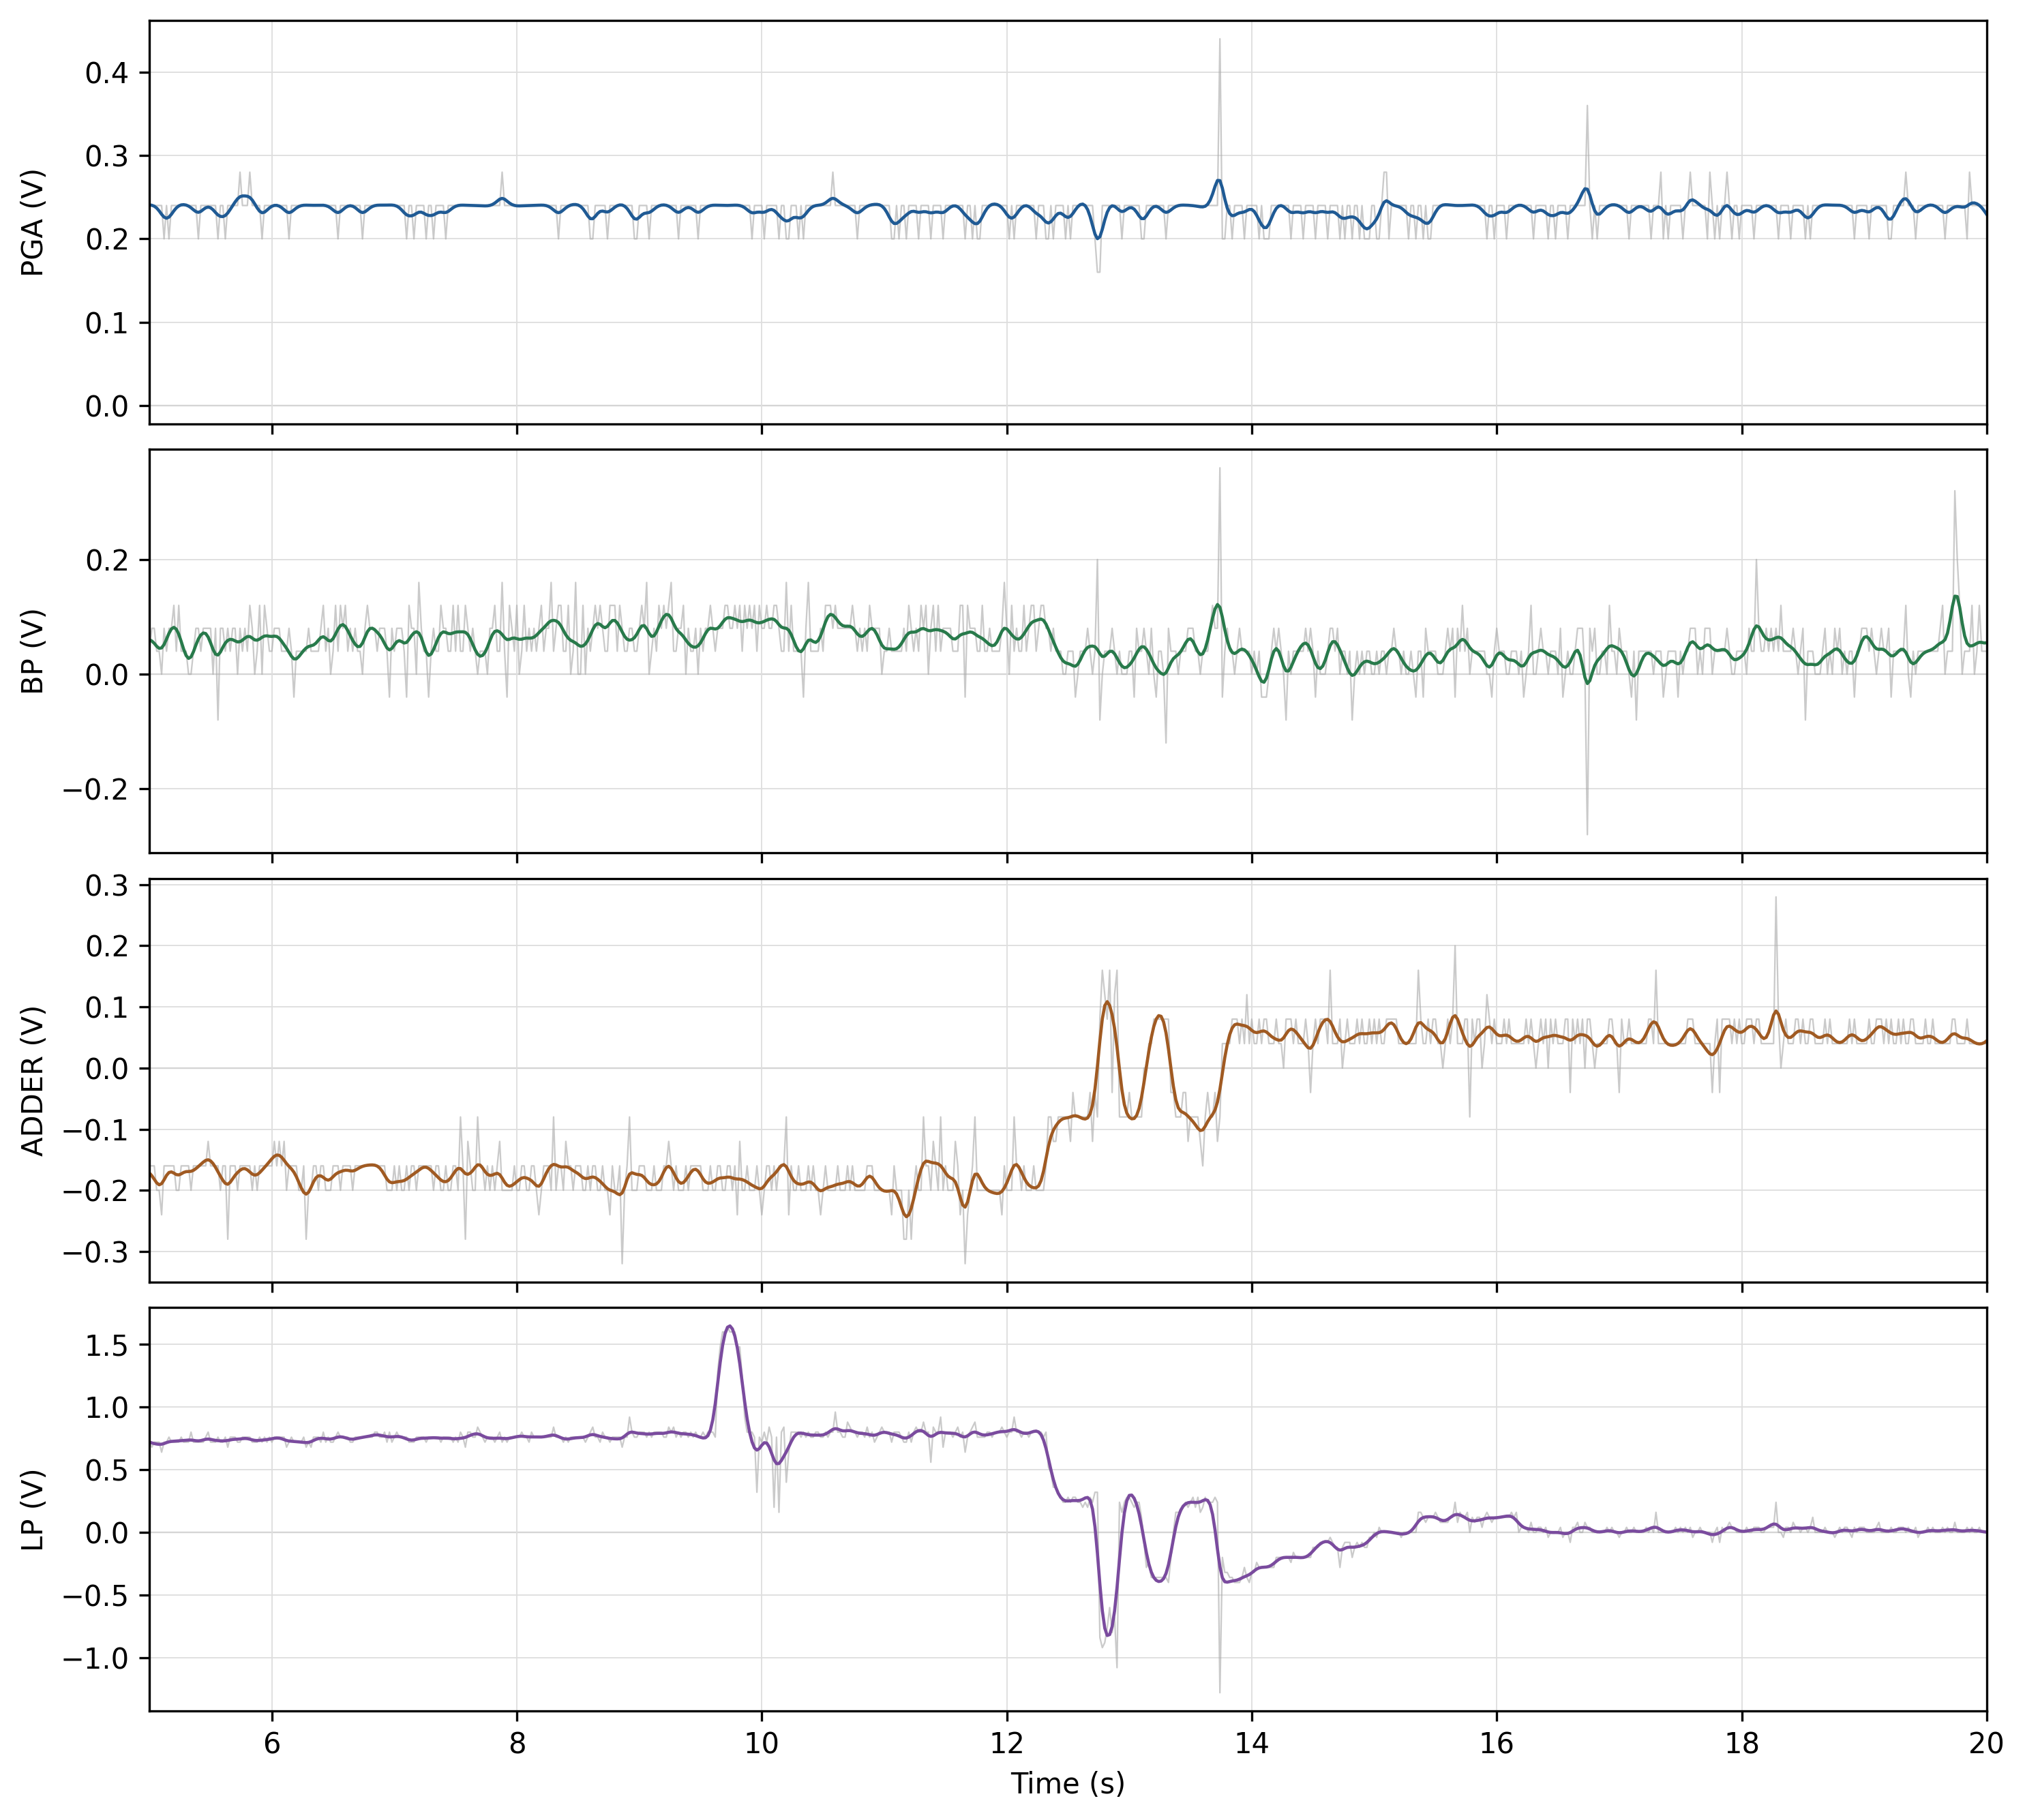
\includegraphics[width=0.88\textwidth,keepaspectratio]{f_senales_por_etapa.png}
\caption{Salidas internas durante una calibración. Las curvas muestran el asentamiento de los ajustes de continua de cada etapa, no una respuesta del terreno.}
\label{fig:calibracion-etapas}
\end{figure*}

\subsection{Caracterización del frente}

Para verificar el comportamiento eléctrico se aplicaron varios barridos senoidales superpuestos y se midieron simultáneamente las salidas internas. Los cocientes espectrales entre entrada y salida permiten estimar magnitud y fase sin depender de la amplitud absoluta del generador; la coherencia se utiliza para descartar puntos dominados por el piso de medición. Se caracterizaron la rama pasabanda, el compensador, el pasa-bajos y la ruta completa hasta el ADC.

Los barridos cubrieron bandas superpuestas desde \SI{10}{mHz} hasta \SI{200}{kHz}. La interpretación se restringió a las zonas con amplitud y coherencia suficientes; extender una curva fuera de ellas confundiría la respuesta del instrumento con el piso de medición. Se identificó la ruta completa PGA--ADC y, por separado, la rama de compensación respecto de la salida del PGA. La comparación por cociente elimina la amplitud absoluta del generador y permite observar tanto la ganancia como el desfase añadido por cada ruta.

\begin{figure*}[!tb]
\centering
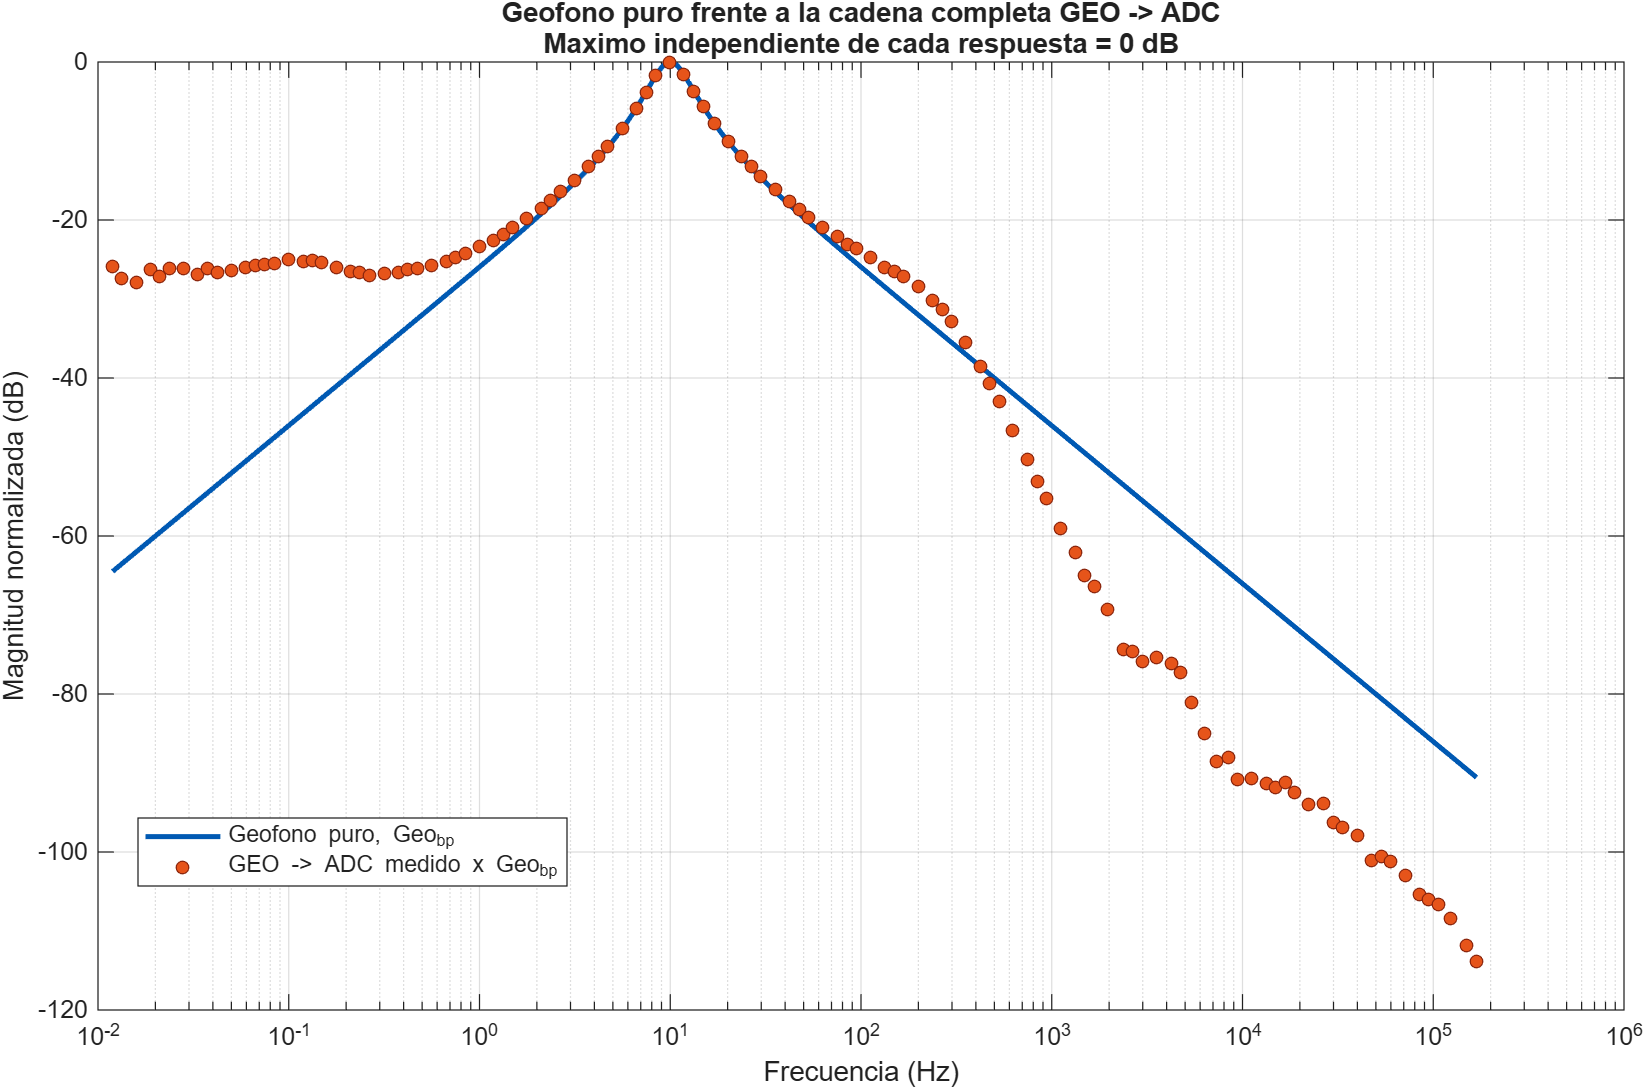
\includegraphics[width=0.88\textwidth]{f_respuesta_geofono_adc.png}
\caption{Comparación normalizada entre el modelo nominal del SM-24 y la respuesta prevista al combinarlo con la transferencia eléctrica medida hasta el ADC. La extensión en baja frecuencia es una predicción de la cadena, no una calibración mecánica.}
\label{fig:caracterizacion-electrica}
\end{figure*}

Los barridos verifican la transferencia eléctrica y el margen de ajuste del potenciómetro. La respuesta geófono--ADC se obtiene combinando esa medición con el modelo nominal del SM-24. No se dispuso de un excitador mecánico trazable capaz de imponer un movimiento conocido al geófono; por ello la cadena completa se presenta como predicción sustentada por ambas partes y no como calibración mecánica extremo a extremo.

\subsection{Asistencia digital y captura de un punto}
\label{sec:digital}

La calibración automática ya requiere multiplexores, ADC, DAC y una secuencia de control; los mismos recursos digitales se aprovechan después para obtener una traza trazable. El convertidor delta--sigma digitaliza la salida del filtro analógico. El traslado de muestras no depende de la atención del procesador: un canal DMA lleva la salida del ADC a memoria, otro la conduce al filtro digital implementado en hardware y un tercero almacena la salida filtrada. El procesador configura la captura y decide qué ruta se conserva, pero no copia muestra por muestra \citep{InfineonPSoC}.

En el prototipo se configuró el ADC delta--sigma a \SI{2604}{muestras/s} y 18 bits nominales, con rangos bipolares de $\pm2{,}5$, $\pm1{,}024$, $\pm0{,}625$ y $\pm0{,}512$ V; la hoja de datos documenta las capacidades del bloque utilizado \citep{InfineonPSoC}. Para un rango $\pm V_R$ y $B$ bits, el paso ideal es
\begin{equation}
q_{\mathrm{ADC}}=\frac{2V_R}{2^B}.
\label{eq:cuantizacion}
\end{equation}
En $\pm\SI{2.5}{V}$ resulta aproximadamente \SI{19.1}{\micro V} por código. Este número es resolución nominal, no ruido medido ni número efectivo de bits. La elección de rango se coordina con la ganancia para aprovechar la escala disponible.

Un promedio y diezmado entero $D$ permite intercambiar banda por duración de captura:
\begin{equation}
y_D[k]=\frac{1}{D}\sum_{m=0}^{D-1}x[kD+m],
\qquad f_{s,\mathrm{sal}}=\frac{2604}{D}\ \mathrm{Hz}.
\label{eq:diezmado}
\end{equation}
El factor utilizado debe conservar la banda de interés y contar con atenuación suficiente antes de la nueva frecuencia de Nyquist. Todos estos parámetros acompañan el archivo para que el eje temporal pueda reconstruirse sin depender de la interfaz que realizó la descarga.

\begin{figure*}[!tb]
\centering
\begin{tikzpicture}[node distance=8mm and 9mm,>=Latex,font=\footnotesize,
  block/.style={draw,rounded corners,minimum height=8mm,minimum width=19mm,align=center,fill=blue!6},
  mem/.style={draw,minimum height=8mm,minimum width=20mm,align=center,fill=green!8}]
  \node[block] (adc) {ADC\\$\Delta\Sigma$};
  \node[block,right=of adc] (dma1) {DMA\\ADC--RAM};
  \node[mem,right=of dma1] (raw) {RAM\\cruda};
  \node[block,below=of dma1] (dma2) {DMA\\ADC--FIR};
  \node[block,right=of dma2] (fir) {FIR\\128 taps};
  \node[block,right=of fir] (dma3) {DMA\\FIR--RAM};
  \node[mem,right=of dma3] (filt) {RAM\\filtrada};
  \draw[->,thick] (adc)--(dma1)--(raw);
  \draw[->,thick] (adc.south) |- (dma2.west);
  \draw[->,thick] (dma2)--(fir)--(dma3)--(filt);
  \node[draw,dashed,rounded corners,fit=(adc)(dma1)(raw)(dma2)(fir)(dma3)(filt),inner sep=5mm,label=below:{lógica: disparo, conteo y cierre; CPU: configuración y metadatos}] {};
\end{tikzpicture}
\caption{Ruta digital implementada en el PSoC. Tres canales DMA trasladan muestras crudas y filtradas sin que el procesador copie cada muestra.}
\label{fig:hardware-digital}
\end{figure*}

Una máquina de estados en lógica programable coordina el disparo, la habilitación del convertidor, el conteo de muestras y el cierre de la ventana. De este modo la duración y el instante de inicio no dependen de latencias variables del firmware. Al finalizar, el bloque informa el estado al procesador, que añade metadatos y escribe el registro en almacenamiento local. La copia local desacopla la integridad de la captura de eventuales pérdidas o demoras de la comunicación inalámbrica.

Para el nodo $i$, con reloj $f_{s,i}=f_s(1+\epsilon_i)$, el tiempo de la muestra $n$ es
\begin{equation}
t_i[n]=t_{0,i}+\frac{n}{f_s(1+\epsilon_i)}.
\label{eq:tiempo-muestra}
\end{equation}
La lógica dedicada estabiliza el conteo local y retira la latencia del procesador, pero no elimina la diferencia de arranque $t_{0,i}-t_{0,j}$ ni la deriva asociada a $\epsilon_i-\epsilon_j$. Ambas deben medirse entre placas. Esta separación evita presentar determinismo interno como si fuera sincronización multicanal validada.

\subsection{Fuente instrumentada e interfaz de campo}
\label{sec:fuente-interfaz}

\paragraph{Fuente instrumentada.} La excitación se aplica con un martillo PCB 086D20 cuyo sensor ICP registra la forma y el instante del impacto. Su banda excede la requerida para localizar el contacto; el acondicionamiento aporta excitación de corriente, elimina la polarización y adapta la señal al ADC \citep{PCB086D20,PCBSignalConditioning}. El nodo HAMMER se implementó con el mismo tipo de PSoC que el receptor y actúa como otro nodo de la red.

El registro completo permite distinguir un golpe único de rebotes o contactos múltiples y comparar realizaciones antes de promediar. La referencia del impacto alinea las capturas secuenciales, pero no sustituye una prueba de sincronización entre ADC de nodos diferentes.

\paragraph{Interfaz e ingesta.} La interfaz web del maestro permite armar los nodos, iniciar la captura y revisar las señales de martillo y geófono. Cada registro incluye la identificación del nodo, la configuración de ganancia y filtrado, la tasa de muestreo y la geometría declarada. La descarga local es opcional: el operador puede conservarla, descartarla antes del procesamiento o enviarla al servidor, cuya ingesta automática valida el paquete, preserva el original y genera derivados sin sobrescribir la medición de campo.

La revisión inmediata cumple una función instrumental: permite detectar saturación, ausencia de acoplamiento, un golpe doble o un nivel de ruido excesivo cuando todavía es posible repetir la posición. No reemplaza el procesamiento posterior. Al descargar, el servidor valida la estructura del archivo, mantiene el original inmutable y asocia las transformaciones con sus parámetros. Así, una nueva selección de golpes o de filtros puede repetirse sin alterar la evidencia adquirida.

Cada sesión se identifica mediante una campaña y cada archivo mediante nodo, posición y número de captura. El encabezado conserva tipo de canal, frecuencia de muestreo, factor de diezmado, rango del ADC, ganancia, ruta cruda o filtrada, cantidad de muestras y estado de calibración. La geometría se almacena como dato de la campaña y se asocia al registro antes de formar el waterfall. Sin esa relación, una traza eléctricamente válida no puede utilizarse para calcular propagación.

La separación entre original y derivado también protege la trazabilidad. El archivo descargado no se reescribe: la alineación fina, el rechazo de golpes, el promediado y la normalización generan resultados nuevos vinculados con su configuración. De esta manera puede establecerse si una diferencia en el waterfall proviene del terreno, de la selección de datos o de un parámetro de procesamiento.

\begin{figure*}[!tb]
\centering
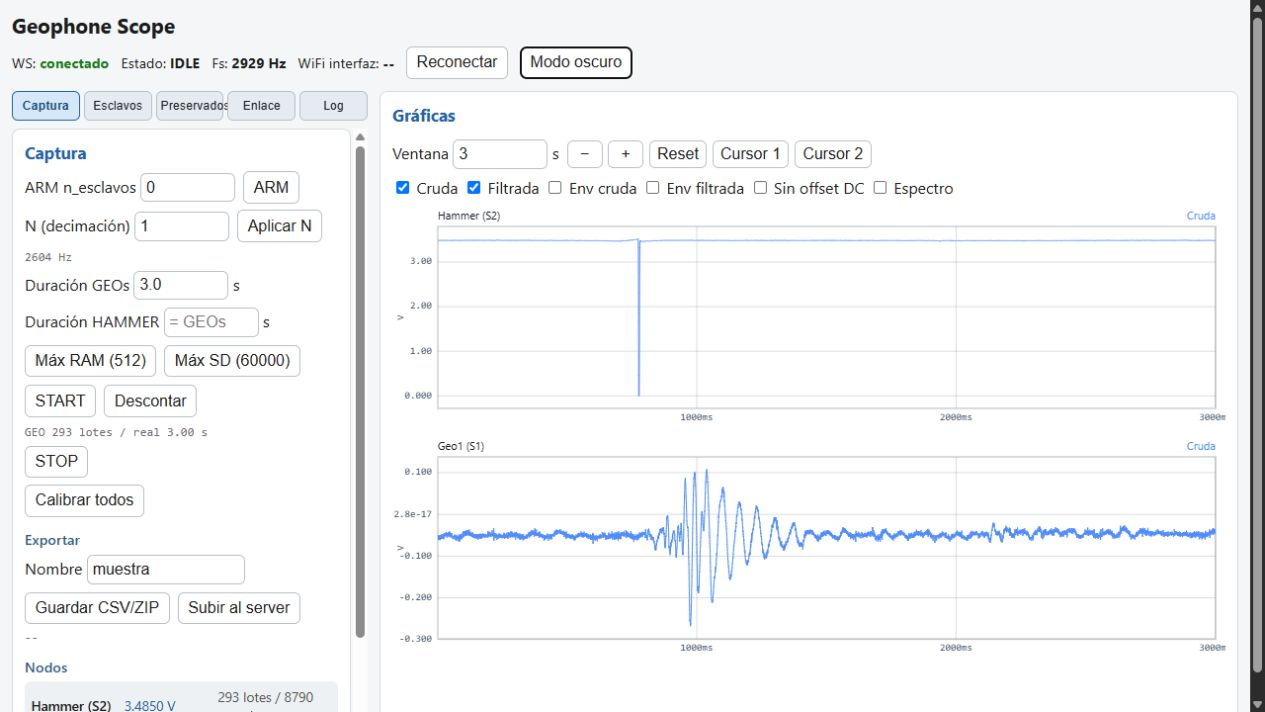
\includegraphics[width=0.88\textwidth,keepaspectratio]{i_web_maestro_claro.png}
\caption{Interfaz del nodo maestro durante la operación: configuración, adquisición y revisión inmediata de las señales recibidas.}
\label{fig:interfaz-campo}
\end{figure*}

\subsection{Arquitectura de múltiples nodos}
\label{sec:multicanal}

La arquitectura admite un maestro, varios nodos GEO y un nodo HAMMER. El maestro envía primero una orden de armado y comprueba que los esclavos estén preparados; después transmite una única orden de inicio por difusión. Cada esclavo genera localmente el flanco que dispara su PSoC, por lo que el muestreo no queda gobernado por la llegada individual de paquetes. La captura termina y se almacena dentro de cada nodo antes de transferirse.

\begin{figure*}[!tb]
\centering
\begin{tikzpicture}[node distance=8mm and 13mm,>=Latex,font=\footnotesize,
  block/.style={draw,rounded corners,minimum height=9mm,minimum width=24mm,align=center,fill=blue!6},
  nodebox/.style={draw,rounded corners,minimum height=12mm,minimum width=35mm,align=center,fill=green!8}]
  \node[block] (ui) {interfaz\\de campo};
  \node[block,right=of ui] (master) {ESP32\\maestro};
  \node[nodebox,right=16mm of master,yshift=8mm] (geo) {nodo GEO\\ESP32 + PSoC + memoria};
  \node[nodebox,right=16mm of master,yshift=-8mm] (hammer) {nodo HAMMER\\ESP32 + PSoC + memoria};
  \draw[<->,thick] (ui)--node[above]{WiFi}(master);
  \draw[<->,thick] (master)--node[above,sloped]{ESP-NOW}(geo);
  \draw[<->,thick] (master)--node[below,sloped]{ESP-NOW}(hammer);
  \node[below=17mm of master,align=center] (seq) {ARM $\rightarrow$ preparación local $\rightarrow$ ACK $\rightarrow$ START común\\$\rightarrow$ captura y almacenamiento local $\rightarrow$ transferencia};
  \draw[->,dashed] (master)--(seq);
\end{tikzpicture}
\caption{Arquitectura distribuida y secuencia de operación. Los nodos se arman antes del START y conservan localmente cada captura antes de transferirla.}
\label{fig:arquitectura-multicanal}
\end{figure*}

El enlace inalámbrico utiliza ESP-NOW, que permite intercambio directo entre dispositivos sin un punto de acceso convencional \citep{EspressifESPNow}. Se separan mensajes de orden, confirmación y transferencia; los datos permanecen respaldados si una entrega falla. El protocolo multiesclavo está implementado y fue sometido a una primera prueba temporal con marcadores GPIO. Esa prueba se presenta en la sección~\ref{sec:resultados}; caracteriza la ejecución del START en los ESP32, no el comienzo efectivo del muestreo en varios ADC.

La transferencia se realiza después de cerrar la ventana. Cada captura queda almacenada en el nodo y se divide en lotes numerados que pueden solicitarse otra vez si el enlace falla. Versiones, CRC e indicadores de cantidad de muestras, desbordamiento y cierre incompleto permiten distinguir una traza íntegra de un archivo parcial. Esta política prioriza la conservación del original sobre la velocidad de descarga.

El armado en dos tiempos reduce el trabajo pendiente en el instante crítico. Primero cada esclavo reserva memoria, configura el PSoC y confirma que espera el disparo. Sólo entonces el maestro difunde la orden común. El esquema evita órdenes sucesivas a cada receptor y reduce la dispersión de inicio; una prueba posterior con una señal analógica común permitirá medir por separado el desfase inicial de los ADC y la deriva de sus relojes.

Duración, tasa, ganancia, rango y ruta se aplican antes del armado y se confirman nodo por nodo. Si alguno no puede reservar memoria, restaurar su calibración o armar el convertidor, la sesión no se declara completa. Identificadores de sesión y secuencia impiden mezclar confirmaciones tardías, archivos parciales o lotes duplicados con una captura válida.

\subsection{Integración de la plataforma}
\label{sec:integracion}

La plataforma integra dos recorridos que se encuentran en una misma sesión. En el nodo GEO, el movimiento vertical atraviesa el geófono, el frente compensado, el ADC y las rutas DMA hasta la memoria local. En el nodo HAMMER, el impacto se acondiciona y digitaliza para proporcionar una referencia de cada excitación. El ESP32 de cada nodo recibe la configuración, arma el PSoC y conserva la captura; el maestro coordina el conjunto y presenta las señales al operador.

La operación comienza al seleccionar duración, tasa, rango, ganancia y ruta de señal. El maestro envía ARM y cada esclavo reserva memoria, restaura su calibración y prepara la adquisición. Sólo después de recibir las confirmaciones se difunde START. El PSoC ejecuta localmente el disparo, el conteo y el cierre, de modo que la transferencia inalámbrica ocurre fuera de la ventana crítica de muestreo.

La división de funciones conserva el determinismo donde resulta necesario. El PSoC gobierna el multiplexor, el ADC, el FIR, los canales DMA y el número exacto de muestras; el ESP32 atiende configuración, estados, comunicación y entrega. Así, una consulta de la interfaz o una retransmisión no modifica el espaciado local de la traza. El final de la ventana queda indicado por la lógica y sólo entonces el procesador prepara los metadatos y habilita el vaciado.

Cada orden pertenece a una sesión identificada. Antes de aceptar START, el esclavo comprueba que la configuración recibida coincide con la memoria reservada y con el estado del PSoC. Los lotes de datos conservan nodo, secuencia y control de integridad; si una entrega se pierde, puede solicitarse nuevamente sin repetir la adquisición. Esta política desacopla la calidad temporal del muestreo de la latencia variable del enlace inalámbrico.

Al concluir la captura, los nodos mantienen el original en almacenamiento local y lo entregan en lotes numerados con control de integridad. La interfaz permite revisar inmediatamente saturación, ausencia de señal o golpes múltiples. Si el registro se conserva, la ingesta automática asocia las trazas, la referencia del impacto, la geometría y los parámetros de adquisición; si se descarta, no se incorpora al procesamiento posterior.

La geometría se incorpora como parte de la sesión y no se infiere del nombre del archivo. Para cada traza se conservan posición, tipo de nodo, tasa de muestreo, rango del ADC, ganancia, ruta cruda o filtrada y estado de calibración. El original permanece inmutable; alineación, promediado, normalización y representación generan derivados asociados a sus parámetros. Esto permite repetir el análisis sin alterar la evidencia adquirida.

Esta integración permite pasar de una captura puntual a dos formas de extensión. La primera repite el mismo nodo GEO en posiciones conocidas y sintetiza un registro espacial. La segunda incorpora varios nodos GEO a la red y conserva la misma secuencia de armado y transferencia. La implementación soporta ambas rutas; la primera produjo el waterfall presentado en este trabajo y la segunda cuenta con una prueba preliminar del START entre tres esclavos.

En la adquisición secuencial, el nodo HAMMER aporta el origen temporal de cada repetición y permite reconocer golpes múltiples antes de formar el promedio. En la adquisición con varios GEO, el mismo HAMMER sigue asociando la respuesta con la excitación, mientras que el START común reduce las diferencias de arranque. Son referencias complementarias: la primera describe cuándo ocurrió el impacto y la segunda coordina los nodos; ninguna permite por sí sola deducir la equivalencia entre sus relojes ADC.

El alcance logrado es, por tanto, el de una plataforma orientada a MASW verificada por subsistemas: el frente fue caracterizado eléctricamente, la calibración y la captura digital operan en el PSoC, y la coordinación e ingesta permiten organizar registros de campo. La equivalencia temporal y metrológica extremo a extremo entre varios receptores constituye el paso experimental siguiente.
